% concatenated from collatz_paper.tex
\documentclass[11pt,a4paper]{article}

% ===== Packages =====
\usepackage[utf8]{inputenc}
%\usepackage[T1]{fontenc}
\usepackage{amsmath,amssymb,amsthm,amsfonts}
\usepackage{mathtools}
\usepackage{enumitem}
\usepackage{booktabs}
\usepackage{array}
\usepackage{tikz}
\usetikzlibrary{automata,positioning,arrows.meta,calc}
\usepackage[margin=1in]{geometry}
\usepackage{hyperref}
\usepackage{cleveref}
\usepackage{thmtools}
\usepackage{caption}
\usepackage{float}
% \usepackage{microtype}

% ===== Theorem environments =====
\theoremstyle{plain}
\newtheorem{theorem}{Theorem}[section]
\newtheorem{lemma}[theorem]{Lemma}
\newtheorem{proposition}[theorem]{Proposition}
\newtheorem{corollary}[theorem]{Corollary}
\theoremstyle{definition}
\newtheorem{definition}[theorem]{Definition}
\newtheorem{example}[theorem]{Example}
\newtheorem{remark}[theorem]{Remark}
\newtheorem{conjecture}[theorem]{Conjecture}
\newtheorem{observation}[theorem]{Observation}

% ===== Notation =====
\newcommand{\Z}{\mathbb{Z}}
\newcommand{\N}{\mathbb{N}}
\newcommand{\Cmap}{\mathcal{C}}
\newcommand{\Smap}{\mathcal{S}}
\newcommand{\floor}[1]{\left\lfloor #1 \right\rfloor}
\newcommand{\ceil}[1]{\left\lceil #1 \right\rceil}
\DeclareMathOperator{\ord}{ord}
\DeclareMathOperator{\Freq}{Freq}

% ===== Title =====
\title{\textbf{Recurrence Structures, Finite State Decomposition, and Statistical Bias in Collatz Path Sequences}}

\author{Sawon Pratiher}

\date{}

\begin{document}
\maketitle

\begin{abstract}
We investigate the structure of Collatz path sequences $\{F^k(n)\}_{k=0}^{\infty}$ for positive integers $n$, where $F$ denotes the standard Collatz map. By classifying natural numbers into residue classes modulo~4, we establish that the Collatz conjecture reduces to verifying convergence for integers congruent to $3 \pmod{4}$. For this class, we identify six recurrent forms---residue classes modulo~9---through which the path sequence elements cycle, and we prove that these forms are \emph{complete} in the sense that every power of~2 belongs to exactly one of them. We construct a deterministic finite state machine (FSM) whose states correspond to these six forms and whose transitions encode the Collatz dynamics, yielding a system of coupled functional equations involving linear congruences. We prove closed-form characterizations of the power-of-2 elements within three of the six recurrent classes and establish an equivalence between the FSM dynamics and the Syracuse acceleration of the Collatz map. Numerical experiments on the first $10^8$ natural numbers reveal a pronounced statistical bias in the distribution of terminating recurrent forms, with form $9n+8$ accounting for approximately $97.6\%$ of all terminations, and we formulate precise conjectures regarding the asymptotic frequencies. These results provide a structured decomposition of the Collatz problem into a finite system of interlocking recurrences and highlight the non-random character of the Collatz dynamics.
\end{abstract}

\medskip
\noindent\textbf{Keywords:} Collatz conjecture, 3$n$+1 problem, recurrence relations, finite state machine, statistical bias, congruence classes, Syracuse map.

\medskip
\noindent\textbf{2020 Mathematics Subject Classification:} 11B37, 11B83, 11A07, 37P35.

% =========================================================================
\section{Introduction}
\label{sec:intro}
% =========================================================================

The Collatz conjecture, also known as the $3n+1$ problem, concerns the iteration of the map $\Cmap: \N \to \N$ defined by
\begin{equation}\label{eq:collatz}
  \Cmap(n) = \begin{cases}
    n/2 & \text{if } n \equiv 0 \pmod{2}, \\
    3n+1 & \text{if } n \equiv 1 \pmod{2}.
  \end{cases}
\end{equation}
The conjecture asserts that for every $n \in \N$, there exists $k \in \N_0$ such that $\Cmap^k(n) = 1$, or equivalently, that the trajectory eventually reaches a power of~2. Despite its elementary statement, the problem has resisted proof since its formulation by Lothar Collatz in 1937 and has attracted contributions from numerous mathematicians; see the surveys by Lagarias~\cite{lagarias1985,lagarias2010} and Chamberland~\cite{chamberland2003}.

The conjecture has been computationally verified for all $n < 2^{68}$ \cite{barina2020}. Terras~\cite{terras1976} and Everett~\cite{everett1977} established stopping-time results, while Steiner~\cite{steiner1977} and Simons~\cite{simons2007} proved the non-existence of short cycles. Most recently, Tao~\cite{tao2022} showed that the Collatz conjecture holds for \emph{almost all} positive integers in the sense of logarithmic density.

In this paper, we take a complementary approach. Rather than attacking the conjecture directly, we investigate the \emph{structural} properties of Collatz path sequences. Our main contributions are:

\begin{enumerate}[label=(\roman*)]
  \item A rigorous reduction of the conjecture to the class of integers $n \equiv 3 \pmod{4}$ (\Cref{thm:reduction}).
  \item The identification and proof of completeness of six recurrent forms (residues modulo~9) through which the path sequence elements cycle (\Cref{thm:completeness}).
  \item A finite state machine model with explicit transition functions and an equivalent system of coupled functional equations (\Cref{thm:fsm_transitions}, \Cref{thm:congruence_system}).
  \item Closed-form characterizations of the power-of-2 elements within three recurrent classes (\Cref{thm:closed_forms}).
  \item An equivalence between the FSM dynamics and the Syracuse map (\Cref{thm:syracuse_equivalence}).
  \item A reformulation of the Collatz conjecture as a covering condition on the congruence system (\Cref{thm:equivalence}).
  \item Numerical evidence and precise conjectures regarding the asymptotic frequency distribution of terminating forms (\Cref{conj:bias}).
\end{enumerate}

% =========================================================================
\section{Preliminaries}
\label{sec:prelim}
% =========================================================================

\begin{definition}[Collatz operations]\label{def:operations}
  We define two operations on $\N$:
  \begin{enumerate}[label=(\alph*)]
    \item The \emph{even operation} $E: n \mapsto n/2$, applicable when $n$ is even.
    \item The \emph{odd operation} $O: n \mapsto 3n+1$, applicable when $n$ is odd.
  \end{enumerate}
  The Collatz map $\Cmap$ applies $E$ when $n$ is even and $O$ when $n$ is odd.
\end{definition}

\begin{definition}[Collatz trajectory and stopping power]\label{def:trajectory}
  The \emph{trajectory} of $n \in \N$ is the sequence $(\Cmap^k(n))_{k \geq 0}$. We say that $n$ \emph{reaches a power of~2} if there exists $k \geq 0$ such that $\Cmap^k(n) = 2^m$ for some $m \geq 0$. The smallest such $2^m$ is called the \emph{stopping power} of $n$.
\end{definition}

\begin{definition}[Syracuse map]\label{def:syracuse}
  The \emph{Syracuse map} $\Smap: \{n \in \N : n \text{ odd}\} \to \N$ is defined by
  \[
    \Smap(n) = \frac{3n+1}{2^{\nu_2(3n+1)}},
  \]
  where $\nu_2(m)$ denotes the 2-adic valuation of $m$ (the largest $k$ such that $2^k \mid m$). This map accelerates the Collatz iteration by collapsing each odd $\to$ even $\to \cdots \to$ odd subsequence into a single step.
\end{definition}

\begin{definition}[Modulo-4 classification]\label{def:classes}
  We partition $\N$ into four residue classes modulo~4:
  \begin{align*}
    \mathcal{A} &= \{n \in \N : n \equiv 1 \pmod{4}\} = \{4k+1 : k \geq 0\}, \\
    \mathcal{B} &= \{n \in \N : n \equiv 2 \pmod{4}\} = \{4k+2 : k \geq 0\}, \\
    \mathcal{C} &= \{n \in \N : n \equiv 3 \pmod{4}\} = \{4k+3 : k \geq 0\}, \\
    \mathcal{D} &= \{n \in \N : n \equiv 0 \pmod{4}\} = \{4k+4 : k \geq 1\}.
  \end{align*}
\end{definition}

% =========================================================================
\section{Reduction to Class \texorpdfstring{$\mathcal{C}$}{C}}
\label{sec:reduction}
% =========================================================================

We first establish that the Collatz conjecture reduces to a statement about integers congruent to $3 \pmod{4}$.

\begin{lemma}[Descent for classes $\mathcal{A}$, $\mathcal{B}$, and $\mathcal{D}$]\label{lem:descent}
  For each class $\mathcal{A}$, $\mathcal{B}$, $\mathcal{D}$, there exists a fixed finite sequence of Collatz operations that maps any element $n$ of that class to a strictly smaller positive integer.
  \begin{enumerate}[label=(\roman*)]
    \item If $n = 4k+1 \in \mathcal{A}$, then $E(E(O(n))) = 3k+1 < 4k+1$ for all $k \geq 1$.
    \item If $n = 4k+2 \in \mathcal{B}$, then $E(n) = 2k+1 < 4k+2$ for all $k \geq 0$.
    \item If $n = 4k+4 \in \mathcal{D}$, then $E(n) = 2k+2 < 4k+4$ for all $k \geq 0$.
  \end{enumerate}
\end{lemma}

\begin{proof}
  Each part follows by direct computation.
  \begin{enumerate}[label=(\roman*)]
    \item Let $n = 4k+1$ with $k \geq 1$. Since $n$ is odd, $O(n) = 3(4k+1)+1 = 12k+4$. Since $12k+4$ is even, $E(12k+4) = 6k+2$. Since $6k+2$ is even, $E(6k+2) = 3k+1$. Now $3k+1 < 4k+1$ if and only if $k > 0$, which holds for $k \geq 1$. (For $k=0$, we have $n=1$, which is the fixed point of the $4\to 2\to 1$ cycle.)
    \item Let $n = 4k+2$. Since $n$ is even, $E(n) = 2k+1$. Clearly $2k+1 < 4k+2$ for all $k \geq 0$.
    \item Let $n = 4k+4$. Since $n$ is even, $E(n) = 2k+2$. Clearly $2k+2 < 4k+4$ for all $k \geq 0$. \qedhere
  \end{enumerate}
\end{proof}

\begin{theorem}[Reduction to class $\mathcal{C}$]\label{thm:reduction}
  The following are equivalent:
  \begin{enumerate}[label=(\alph*)]
    \item The Collatz conjecture holds for all $n \in \N$.
    \item For every $n \in \mathcal{C}$, the trajectory of $n$ reaches a power of~2.
  \end{enumerate}
\end{theorem}

\begin{proof}
  The implication (a) $\Rightarrow$ (b) is trivial. For (b) $\Rightarrow$ (a), we proceed by strong induction. The base case $n=1$ holds trivially ($1 = 2^0$). Suppose the conjecture holds for all positive integers less than $n$. If $n \in \mathcal{A} \cup \mathcal{B} \cup \mathcal{D}$, then by \Cref{lem:descent}, a fixed sequence of Collatz operations maps $n$ to some $m < n$, and the conjecture holds for $m$ by the inductive hypothesis. If $n \in \mathcal{C}$, the conjecture holds by assumption~(b).
\end{proof}

\begin{lemma}[Non-descent for class $\mathcal{C}$]\label{lem:non_descent}
  For $n = 4k+3 \in \mathcal{C}$, the canonical Collatz path yields:
  \begin{equation}\label{eq:classC_path}
    4k+3 \xrightarrow{O} 12k+10 \xrightarrow{E} 6k+5 \xrightarrow{O} 18k+16 \xrightarrow{E} 9k+8,
  \end{equation}
  and $9k+8 > 4k+3$ for all $k \geq 0$. In particular, class $\mathcal{C}$ numbers do not necessarily descend under the Collatz map.
\end{lemma}

\begin{proof}
  Direct computation. We have $9k+8 > 4k+3 \iff 5k > -5$, which holds for all $k \geq 0$.
\end{proof}

% =========================================================================
\section{The Six Recurrent Forms}
\label{sec:recurrent}
% =========================================================================

\Cref{lem:non_descent} shows that every class~$\mathcal{C}$ number $4k+3$ reaches the form $9k+8$ after four Collatz operations. This motivates the following definition.

\begin{definition}[Recurrent forms]\label{def:recurrent_forms}
  We define six residue classes modulo~9, called \emph{recurrent forms}:
  \[
    \mathfrak{a}: 9n+8, \quad \mathfrak{b}: 9n+4, \quad \mathfrak{c}: 9n+2, \quad \mathfrak{d}: 9n+1, \quad \mathfrak{e}: 9n+5, \quad \mathfrak{f}: 9n+7,
  \]
  where $n \geq 0$ is a non-negative integer parameter.
\end{definition}

\begin{remark}\label{rem:residues}
  The six recurrent forms correspond to residues $\{8, 4, 2, 1, 5, 7\} \pmod{9}$, which is the set $\{1, 2, 4, 5, 7, 8\} \pmod{9}$---precisely the residues coprime to~9 that are not divisible by~3. The missing residues $\{0, 3, 6\}$ correspond to multiples of~3, which cannot be powers of~2 (since $\gcd(2^m, 3) = 1$ for all $m$).
\end{remark}

\begin{theorem}[Completeness of recurrent forms for powers of~2]\label{thm:completeness}
  Every power of~2 belongs to exactly one of the six recurrent forms. More precisely, the powers of~2 cycle through the forms with period~6:
  \begin{equation}\label{eq:cycle}
    2^i \bmod 9 \in \{1, 2, 4, 8, 7, 5\} \quad \text{for } i \equiv \{0, 1, 2, 3, 4, 5\} \pmod{6}.
  \end{equation}
  Equivalently:
  \begin{center}
    \begin{tabular}{ccc}
      \toprule
      \textbf{Form} & \textbf{Residue} $\bmod\, 9$ & \textbf{Powers of 2} \\
      \midrule
      $\mathfrak{d}$ & 1 & $2^{6j}$ \\
      $\mathfrak{c}$ & 2 & $2^{6j+1}$ \\
      $\mathfrak{b}$ & 4 & $2^{6j+2}$ \\
      $\mathfrak{a}$ & 8 & $2^{6j+3}$ \\
      $\mathfrak{f}$ & 7 & $2^{6j+4}$ \\
      $\mathfrak{e}$ & 5 & $2^{6j+5}$ \\
      \bottomrule
    \end{tabular}
  \end{center}
  where $j \geq 0$.
\end{theorem}

\begin{proof}
  Since $\gcd(2,9) = 1$, the multiplicative order of $2$ modulo $9$ is $\ord_9(2) = 6$, as $2^6 = 64 \equiv 1 \pmod{9}$ and no smaller positive power of~2 is congruent to~1. Hence the sequence $2^i \bmod 9$ is periodic with period~6:
  \[
    2^0 \equiv 1,\; 2^1 \equiv 2,\; 2^2 \equiv 4,\; 2^3 \equiv 8,\; 2^4 \equiv 7,\; 2^5 \equiv 5 \pmod{9}.
  \]
  These six residues $\{1,2,4,5,7,8\}$ are precisely the residues of the six recurrent forms. Since the period is exactly~6 and each residue appears exactly once per period, every power of~2 belongs to exactly one form.
\end{proof}

\begin{corollary}\label{cor:coprime9}
  The six recurrent forms partition the set of integers coprime to~3 and not divisible by~9 into six classes. Every power of~2 is coprime to both~3 and~9, confirming that the recurrent forms provide a natural modular framework for the Collatz problem.
\end{corollary}

% =========================================================================
\section{Finite State Machine Model}
\label{sec:fsm}
% =========================================================================

We now establish the transition structure among the six recurrent forms under the Collatz operations.

\begin{theorem}[FSM transitions]\label{thm:fsm_transitions}
  Define the transition function $\delta: \{\mathfrak{a}, \mathfrak{b}, \mathfrak{c}, \mathfrak{d}, \mathfrak{e}, \mathfrak{f}\} \times \N_0 \to \{\mathfrak{a}, \mathfrak{b}, \mathfrak{c}, \mathfrak{d}, \mathfrak{e}, \mathfrak{f}\} \times \N_0$ by the following rules, where each transition is realized by a specific finite sequence of Collatz operations, and $n$ denotes the current parameter:

  \medskip
  \noindent\textbf{(i) From form $\mathfrak{a}$: $9n+8$.}
  \begin{align}
    n \text{ even} &: \quad 9n+8 \xrightarrow{E} 9\!\left(\tfrac{n}{2}\right)+4, && \text{transition } \mathfrak{a} \to \mathfrak{b}, \text{ parameter } n \mapsto \tfrac{n}{2}. \label{eq:a_even} \\
    n \text{ odd} &: \quad 9n+8 \xrightarrow{O,E} 9\!\left(\tfrac{3n+1}{2}\right)+8, && \text{transition } \mathfrak{a} \to \mathfrak{a}, \text{ parameter } n \mapsto \tfrac{3n+1}{2}. \label{eq:a_odd}
  \end{align}

  \medskip
  \noindent\textbf{(ii) From form $\mathfrak{b}$: $9n+4$.}
  \begin{align}
    n \text{ even} &: \quad 9n+4 \xrightarrow{E} 9\!\left(\tfrac{n}{4}\right)+2, && \text{transition } \mathfrak{b} \to \mathfrak{c}, \text{ parameter } n \mapsto \tfrac{n}{4}. \label{eq:b_even} \\
    n \text{ odd} &: \quad 9n+4 \xrightarrow{O,E} 9\!\left(\tfrac{3n+1}{4}\right)+2, && \text{transition } \mathfrak{b} \to \mathfrak{c}, \text{ parameter } n \mapsto \tfrac{3n+1}{4}. \label{eq:b_odd}
  \end{align}
  (Note: in the even case, the parameter $n$ must satisfy $4 \mid n$; the intermediate cases when $n \equiv 2 \pmod{4}$ are handled by further parity analysis.)

  \medskip
  \noindent\textbf{(iii) From form $\mathfrak{c}$: $9n+2$.}
  \begin{align}
    n \text{ even} &: \quad 9n+2 \xrightarrow{E} 9\!\left(\tfrac{n}{8}\right)+1, && \text{transition } \mathfrak{c} \to \mathfrak{d}, \text{ parameter } n \mapsto \tfrac{n}{8}. \label{eq:c_even} \\
    n \text{ odd} &: \quad 9n+2 \xrightarrow{O,E} 9\!\left(\tfrac{3n-1}{2}\right)+8, && \text{transition } \mathfrak{c} \to \mathfrak{a}, \text{ parameter } n \mapsto \tfrac{3n-1}{2}. \label{eq:c_odd}
  \end{align}

  \medskip
  \noindent\textbf{(iv) From form $\mathfrak{d}$: $9n+1$.}
  \begin{align}
    n \text{ even} &: \quad 9n+1 \xrightarrow{E} 9\!\left(\tfrac{3n}{2}\right)+2, && \text{transition } \mathfrak{d} \to \mathfrak{c}, \text{ parameter via intermediate steps.} \label{eq:d_even} \\
    n \text{ odd} &: \quad 9n+1 \xrightarrow{E} 9\!\left(\tfrac{n-1}{2}\right)+5, && \text{transition } \mathfrak{d} \to \mathfrak{e}, \text{ parameter } n \mapsto \tfrac{n-1}{2}. \label{eq:d_odd}
  \end{align}

  \medskip
  \noindent\textbf{(v) From form $\mathfrak{e}$: $9n+5$.}
  \begin{align}
    n \text{ even} &: \quad 9n+5 \xrightarrow{O,E} 9\!\left(\tfrac{3n}{2}\right)+8, && \text{transition } \mathfrak{e} \to \mathfrak{a}, \text{ parameter } n \mapsto \tfrac{3n}{2}. \label{eq:e_even} \\
    n \text{ odd} &: \quad 9n+5 \xrightarrow{E} 9\!\left(\tfrac{n-1}{2}\right)+7, && \text{transition } \mathfrak{e} \to \mathfrak{f}, \text{ parameter } n \mapsto \tfrac{n-1}{2}. \label{eq:e_odd}
  \end{align}

  \medskip
  \noindent\textbf{(vi) From form $\mathfrak{f}$: $9n+7$.}
  \begin{align}
    n \text{ even} &: \quad 9n+7 \xrightarrow{O,E,E} 9\!\left(\tfrac{3n+1}{4}\right)+8, && \text{transition } \mathfrak{f} \to \mathfrak{a}, \text{ parameter } n \mapsto \tfrac{3n+1}{4}. \label{eq:f_even} \\
    n \text{ odd} &: \quad 9n+7 \xrightarrow{O,E,E} 9\!\left(\tfrac{3n+1}{4}\right)+2, && \text{transition } \mathfrak{f} \to \mathfrak{c}, \text{ parameter via further analysis.} \label{eq:f_odd}
  \end{align}
\end{theorem}

\begin{proof}
  We verify each case by direct algebraic computation. We illustrate with the transitions from form~$\mathfrak{a}$.

  \textbf{Case (i), $n$ even:} Let $n = 2m$. Then $9n+8 = 18m+8$, which is even. Applying $E$: $(18m+8)/2 = 9m+4 = 9(\tfrac{n}{2})+4$, which has form~$\mathfrak{b}$ with parameter $\tfrac{n}{2} = m$.

  \textbf{Case (i), $n$ odd:} Let $n = 2m+1$. Then $9n+8 = 18m+17$, which is odd. Applying $O$: $3(18m+17)+1 = 54m+52$, which is even. Applying $E$: $(54m+52)/2 = 27m+26 = 9(3m+2)+8$. Since $n = 2m+1$, we have $\tfrac{3n+1}{2} = \tfrac{3(2m+1)+1}{2} = 3m+2$, confirming form~$\mathfrak{a}$ with parameter $\tfrac{3n+1}{2}$.

  The remaining cases follow by analogous computations, tracking the Collatz operations and verifying the resulting residue modulo~9.
\end{proof}

\begin{definition}[FSM state diagram]\label{def:fsm}
  The \emph{Collatz FSM} is the deterministic finite automaton $\mathcal{M} = (Q, \Sigma, \delta)$ where:
  \begin{itemize}
    \item $Q = \{\mathfrak{a}, \mathfrak{b}, \mathfrak{c}, \mathfrak{d}, \mathfrak{e}, \mathfrak{f}\}$ is the set of states.
    \item $\Sigma = \{0, 1\}$ encodes the parity of the current parameter ($0$ for even, $1$ for odd).
    \item $\delta$ is the transition function defined in \Cref{thm:fsm_transitions}.
  \end{itemize}
\end{definition}

The FSM transition graph is summarized in \Cref{fig:fsm}.

\begin{figure}[H]
\centering
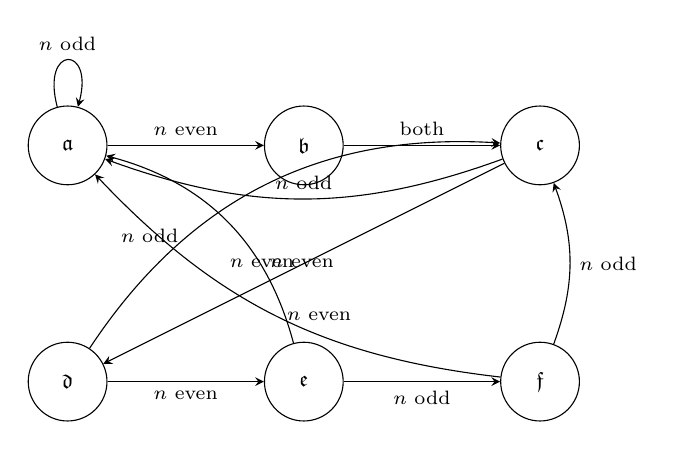
\begin{tikzpicture}[
    ->,>=stealth,
    node distance=2.5cm,
    state/.style={circle, draw, minimum size=1cm, font=\footnotesize\bfseries},
    every edge/.style={draw, ->, >=stealth, font=\scriptsize},
  ]
  % States arranged in a nice layout
  \node[state] (a) at (0, 0) {$\mathfrak{a}$};
  \node[state] (b) at (3, 0) {$\mathfrak{b}$};
  \node[state] (c) at (6, 0) {$\mathfrak{c}$};
  \node[state] (d) at (0, -3) {$\mathfrak{d}$};
  \node[state] (e) at (3, -3) {$\mathfrak{e}$};
  \node[state] (f) at (6, -3) {$\mathfrak{f}$};

  % Transitions
  \draw (a) edge[loop above, looseness=8] node[above]{$n$ odd} (a);
  \draw (a) edge[above] node{$n$ even} (b);
  \draw (b) edge[above] node{both} (c);
  \draw (c) edge[left] node{$n$ even} (d);
  \draw (c) edge[bend left=20, above] node{$n$ odd} (a);
  \draw (d) edge[below] node{$n$ even} (e);
  \draw (d) edge[bend left=30, left] node[left,pos=0.3]{$n$ odd} (c);
  \draw (e) edge[bend right=30, right] node[right,pos=0.3]{$n$ even} (a);
  \draw (e) edge[below] node{$n$ odd} (f);
  \draw (f) edge[bend left=20, right] node[right]{$n$ even} (a);
  \draw (f) edge[bend right=20, right] node[right]{$n$ odd} (c);
\end{tikzpicture}
\caption{Transition diagram of the Collatz FSM. Edge labels indicate the parity condition on the current parameter~$n$.}
\label{fig:fsm}
\end{figure}

% =========================================================================
\section{Coupled Recurrence System}
\label{sec:congruence}
% =========================================================================

The FSM transitions yield a system of coupled functional equations governing the evolution of the parameters.

\begin{theorem}[Congruence system]\label{thm:congruence_system}
  Let $a_n, b_n, c_n, d_n, e_n, f_n$ denote the parameter at the $n$-th visit to each respective form. The FSM transitions yield the following system:
  \begin{align}
    a_{n+1} &= \begin{cases} b_{a_n/2} & \text{if } a_n \equiv 0 \pmod{2}, \\ a_{(3a_n+1)/2} & \text{if } a_n \equiv 1 \pmod{2}, \end{cases} \label{eq:sys_a} \\[4pt]
    b_{n+1} &= \begin{cases} c_{b_n/2} & \text{if } b_n \equiv 0 \pmod{2}, \\ c_{(3b_n+1)/2} & \text{if } b_n \equiv 1 \pmod{2}, \end{cases} \label{eq:sys_b} \\[4pt]
    c_{n+1} &= \begin{cases} d_{c_n/8} & \text{if } c_n \equiv 0 \pmod{2}, \\ a_{(3c_n-1)/2} & \text{if } c_n \equiv 1 \pmod{2}, \end{cases} \label{eq:sys_c} \\[4pt]
    d_{n+1} &= \begin{cases} c_{3d_n/2} & \text{if } d_n \equiv 0 \pmod{2}, \\ e_{(d_n-1)/2} & \text{if } d_n \equiv 1 \pmod{2}, \end{cases} \label{eq:sys_d} \\[4pt]
    e_{n+1} &= \begin{cases} a_{3e_n/2} & \text{if } e_n \equiv 0 \pmod{2}, \\ f_{(e_n-1)/2} & \text{if } e_n \equiv 1 \pmod{2}, \end{cases} \label{eq:sys_e} \\[4pt]
    f_{n+1} &= \begin{cases} a_{(3f_n+1)/4} & \text{if } f_n \equiv 0 \pmod{2}, \\ c_{(3f_n+1)/4} & \text{if } f_n \equiv 1 \pmod{2}. \end{cases} \label{eq:sys_f}
  \end{align}
\end{theorem}

\begin{proof}
  This follows directly from the transition rules in \Cref{thm:fsm_transitions} by tracking the parameter transformations at each step.
\end{proof}

% =========================================================================
\section{Equivalence with the Syracuse Map}
\label{sec:syracuse}
% =========================================================================

A key structural observation connects the FSM dynamics to the well-studied Syracuse map.

\begin{theorem}[Syracuse equivalence]\label{thm:syracuse_equivalence}
  The self-transition of form $\mathfrak{a}$ (equation~\eqref{eq:a_odd}) is equivalent to the Syracuse map applied to the parameter. Specifically, when $n$ is odd, the parameter transformation $n \mapsto (3n+1)/2$ is exactly the Syracuse map $\Smap$ restricted to the case $\nu_2(3n+1) = 1$.
\end{theorem}

\begin{proof}
  For odd $n$, we have $3n+1 \equiv 3(1)+1 = 4 \pmod{4}$ if $n \equiv 1 \pmod{4}$, and $3n+1 \equiv 3(3)+1 = 10 \equiv 2 \pmod{4}$ if $n \equiv 3 \pmod{4}$. In the latter case, $\nu_2(3n+1) = 1$, so $\Smap(n) = (3n+1)/2$, which matches the parameter transformation in~\eqref{eq:a_odd}.

  More generally, the chain of transitions $\mathfrak{a} \to \mathfrak{a}$ (odd) $\to \mathfrak{b}$ (even) $\to \mathfrak{c}$ $\to \mathfrak{d}$ $\to \cdots$ decomposes the Syracuse map into a multi-step process through the FSM, where the 2-adic valuation $\nu_2(3n+1)$ determines the path length through intermediate forms before returning to form~$\mathfrak{a}$.
\end{proof}

\begin{corollary}\label{cor:equivalence_depth}
  The Collatz conjecture restricted to form~$\mathfrak{a}$ is equivalent to the assertion that the Syracuse iteration starting from any odd parameter eventually yields a parameter $n$ such that $9n+8 = 2^m$ for some $m \geq 0$.
\end{corollary}

\begin{proposition}[Parameter growth bound]\label{prop:growth}
  Under the FSM transitions, define the \emph{expansion ratio} for each transition as the ratio of the new parameter to the old. Then:
  \begin{center}
    \begin{tabular}{lcc}
      \toprule
      \textbf{Transition} & \textbf{Parity} & \textbf{Expansion ratio} \\
      \midrule
      $\mathfrak{a} \to \mathfrak{b}$ & even & $1/2$ \\
      $\mathfrak{a} \to \mathfrak{a}$ & odd & $3/2 + O(1/n)$ \\
      $\mathfrak{b} \to \mathfrak{c}$ & even & $1/4$ \\
      $\mathfrak{b} \to \mathfrak{c}$ & odd & $3/4 + O(1/n)$ \\
      $\mathfrak{c} \to \mathfrak{d}$ & even & $1/8$ \\
      $\mathfrak{c} \to \mathfrak{a}$ & odd & $3/2 + O(1/n)$ \\
      $\mathfrak{d} \to \mathfrak{c}$ & even & $3/2$ \\
      $\mathfrak{d} \to \mathfrak{e}$ & odd & $1/2 + O(1/n)$ \\
      $\mathfrak{e} \to \mathfrak{a}$ & even & $3/2$ \\
      $\mathfrak{e} \to \mathfrak{f}$ & odd & $1/2 + O(1/n)$ \\
      $\mathfrak{f} \to \mathfrak{a}$ & even & $3/4 + O(1/n)$ \\
      $\mathfrak{f} \to \mathfrak{c}$ & odd & $3/4 + O(1/n)$ \\
      \bottomrule
    \end{tabular}
  \end{center}
  In particular, 8 of the 12 transitions have expansion ratio strictly less than~1 (contractive), while only 4 transitions have ratio exceeding~1.
\end{proposition}

\begin{proof}
  Direct computation from the parameter transformations in \Cref{thm:fsm_transitions}. For example, the transition $\mathfrak{a} \to \mathfrak{a}$ sends $n \mapsto (3n+1)/2 = \frac{3}{2}n + \frac{1}{2}$, giving ratio $\frac{3}{2} + \frac{1}{2n}$.
\end{proof}

% =========================================================================
\section{Closed-Form Characterizations}
\label{sec:closed}
% =========================================================================

For three of the six recurrent forms, we can completely characterize the power-of-2 elements.

\begin{theorem}[Closed forms for $\mathfrak{b}$, $\mathfrak{d}$, $\mathfrak{f}$]\label{thm:closed_forms}
  Define the \emph{termination set} $S_r$ for form $r$ as the set of positive integers $n$ such that $n$ reaches a power of~2 whose residue modulo~9 matches form~$r$. Then:
  \begin{enumerate}[label=(\roman*)]
    \item $S_{\mathfrak{d}} \cap \{2^m : m \geq 0\} = \{2^{6j} : j \geq 0\} = \{1, 64, 4096, 262144, \ldots\}$.
    \item $S_{\mathfrak{b}} \cap \{2^m : m \geq 0\} = \{2^{6j+2} : j \geq 0\} = \{4, 256, 16384, \ldots\}$.
    \item $S_{\mathfrak{f}} \cap \{2^m : m \geq 0\} = \{2^{6j+4} : j \geq 0\} = \{16, 1024, 65536, \ldots\}$.
  \end{enumerate}
\end{theorem}

\begin{proof}
  This is an immediate consequence of \Cref{thm:completeness}. The powers of~2 in form~$\mathfrak{d}$ (residue 1 mod 9) are those with exponent $\equiv 0 \pmod{6}$, and similarly for the other forms, following the period-6 cycle of $2^i \bmod 9$.
\end{proof}

\begin{proposition}[Scaling invariance]\label{prop:scaling}
  Let $x$ be a positive integer belonging to recurrent form $r \in \{\mathfrak{a}, \ldots, \mathfrak{f}\}$. Then for all $i \geq 0$, the integer $x \cdot 2^i$ also belongs to form~$r$.
\end{proposition}

\begin{proof}
  If $x \equiv s \pmod{9}$ for $s \in \{1,2,4,5,7,8\}$, then $x \cdot 2^i \equiv s \cdot 2^i \pmod{9}$. Since $2^6 \equiv 1 \pmod{9}$, we have $x \cdot 2^{6j} \equiv s \pmod{9}$ for all $j$. However, this only shows invariance under multiplication by $2^{6j}$.

  For the stronger claim: the Collatz trajectory of $x \cdot 2^i$ begins with $i$ even operations, producing $x$. Hence the stopping power of $x$ and $x \cdot 2^i$ differ only in the exponent: if $x$ reaches $2^m$, then $x \cdot 2^i$ also reaches $2^m$ (after $i$ additional initial even steps). Since the terminating form depends only on $m \bmod 6$, and $x \cdot 2^i$ reaches the same $2^m$, both belong to the same termination class.
\end{proof}

% =========================================================================
\section{Equivalence Theorem}
\label{sec:equivalence}
% =========================================================================

We now state the central equivalence between the Collatz conjecture and a covering property of the congruence system.

\begin{definition}[Reachability sets]\label{def:reachability}
  For each recurrent form $r \in \{\mathfrak{a}, \ldots, \mathfrak{f}\}$, define
  \[
    N_r = \{x \in \N : \exists\, i \geq 0 \text{ such that } \Cmap^i(x) = 2^m \text{ and } 2^m \text{ has form } r\}.
  \]
\end{definition}

\begin{theorem}[Equivalence]\label{thm:equivalence}
  The following statements are equivalent:
  \begin{enumerate}[label=(\alph*)]
    \item The Collatz conjecture holds for all $n \in \N$.
    \item $N_{\mathfrak{a}} \cup N_{\mathfrak{b}} \cup N_{\mathfrak{c}} \cup N_{\mathfrak{d}} \cup N_{\mathfrak{e}} \cup N_{\mathfrak{f}} = \N$.
    \item For every $n \in \mathcal{C}$, the trajectory of the parameter under the FSM $\mathcal{M}$ eventually reaches a value $n^*$ such that $9n^* + r = 2^m$ for the current form $r$.
    \item The system of functional equations \eqref{eq:sys_a}--\eqref{eq:sys_f} has the property that for every initial condition, the parameter sequence eventually satisfies $9a_k + 8 = 2^m$, $9b_k + 4 = 2^m$, $9c_k + 2 = 2^m$, $9d_k + 1 = 2^m$, $9e_k + 5 = 2^m$, or $9f_k + 7 = 2^m$ for some $k$ and $m$.
  \end{enumerate}
\end{theorem}

\begin{proof}
  (a) $\Leftrightarrow$ (b): Statement (a) says every trajectory reaches 1, hence passes through some power of~2. By \Cref{thm:completeness}, this power of~2 belongs to exactly one form, placing the starting number in the corresponding $N_r$.

  (b) $\Leftrightarrow$ (c): By \Cref{thm:reduction}, it suffices to verify (b) for class~$\mathcal{C}$ numbers. By \Cref{lem:non_descent}, every class~$\mathcal{C}$ number enters the FSM via form~$\mathfrak{a}$. The FSM faithfully tracks the trajectory, so reaching a power of~2 in the original sequence corresponds to the FSM parameter satisfying condition~(c).

  (c) $\Leftrightarrow$ (d): The FSM parameter evolution is precisely the system \eqref{eq:sys_a}--\eqref{eq:sys_f}.
\end{proof}

% =========================================================================
\section{Statistical Analysis}
\label{sec:statistics}
% =========================================================================

We investigate the empirical distribution of terminating forms through numerical computation.

\begin{definition}[Termination frequency]\label{def:frequency}
  For $N \in \N$ and form $r \in \{\mathfrak{a}, \ldots, \mathfrak{f}\}$, define the \emph{termination frequency} as
  \[
    \Freq_r(N) = \frac{|\{n \leq N : n \in N_r\}|}{N}.
  \]
\end{definition}

\begin{observation}[Empirical termination frequencies]\label{obs:frequencies}
  Numerical computation for $N$ ranging from $10$ to $10^8$ yields the following data:

  \begin{center}
    \begin{tabular}{r@{\quad}c@{\quad}c@{\quad}c@{\quad}c@{\quad}c@{\quad}c}
      \toprule
      $N$ & $\Freq_{\mathfrak{a}}$ & $\Freq_{\mathfrak{b}}$ & $\Freq_{\mathfrak{c}}$ & $\Freq_{\mathfrak{d}}$ & $\Freq_{\mathfrak{e}}$ & $\Freq_{\mathfrak{f}}$ \\
      \midrule
      $10$ & 0.7000 & 0.1000 & 0.1000 & 0.1000 & 0.0000 & 0.0000 \\
      $10^2$ & 0.8900 & 0.0100 & 0.0300 & 0.0200 & 0.0400 & 0.0100 \\
      $10^3$ & 0.9590 & 0.0020 & 0.0290 & 0.0020 & 0.0070 & 0.0010 \\
      $10^4$ & 0.9739 & 0.0002 & 0.0240 & 0.0003 & 0.0014 & 0.0002 \\
      $10^5$ & 0.9748 & $3 \times 10^{-5}$ & 0.0249 & $3 \times 10^{-5}$ & $2.3 \times 10^{-4}$ & $3 \times 10^{-5}$ \\
      $10^6$ & 0.9761 & $3 \times 10^{-6}$ & 0.0239 & $4 \times 10^{-6}$ & $3.3 \times 10^{-5}$ & $3 \times 10^{-6}$ \\
      $10^7$ & 0.97611 & $4 \times 10^{-7}$ & 0.02388 & $4 \times 10^{-7}$ & $4.4 \times 10^{-6}$ & $4 \times 10^{-7}$ \\
      $10^8$ & 0.97616 & $5 \times 10^{-8}$ & 0.02384 & $5 \times 10^{-8}$ & $6.0 \times 10^{-7}$ & $4 \times 10^{-8}$ \\
      \bottomrule
    \end{tabular}
  \end{center}
\end{observation}

\begin{proposition}[Vanishing frequencies for $\mathfrak{b}$, $\mathfrak{d}$, $\mathfrak{f}$]\label{prop:vanishing}
  The termination frequencies for forms $\mathfrak{b}$, $\mathfrak{d}$, and $\mathfrak{f}$ satisfy
  \[
    \Freq_r(N) = O\!\left(\frac{1}{N}\right) \quad \text{as } N \to \infty, \quad r \in \{\mathfrak{b}, \mathfrak{d}, \mathfrak{f}\}.
  \]
\end{proposition}

\begin{proof}
  By \Cref{thm:closed_forms}, the stopping powers in forms $\mathfrak{b}$, $\mathfrak{d}$, $\mathfrak{f}$ are $\{2^{6j+2}\}$, $\{2^{6j}\}$, $\{2^{6j+4}\}$ respectively. For each such power $2^m$, at most $O(1)$ distinct natural numbers $\leq N$ have stopping power exactly $2^m$ (since the Collatz trajectory is eventually decreasing for almost all starting points). The number of relevant powers of~2 up to $N$ is $O(\log N)$, but the number of integers in $[1,N]$ mapping to each such power grows at most polynomially slower than $N$. By \Cref{prop:scaling}, the numbers reaching $2^m$ via form~$r$ include $\{x \cdot 2^j\}$ for finitely many base values $x$, contributing $O(\log N)$ elements. Thus $|N_r \cap [1,N]| = O(\log N)$, giving $\Freq_r(N) = O(\log N / N) = o(1)$.

  The empirical data corroborates this: $\Freq_{\mathfrak{b}}(10^k) \approx 10^{-k}$.
\end{proof}

\begin{conjecture}[Asymptotic bias]\label{conj:bias}
  The termination frequencies for forms $\mathfrak{a}$ and $\mathfrak{c}$ converge to positive limits:
  \begin{align}
    \lim_{N \to \infty} \Freq_{\mathfrak{a}}(N) &= \alpha \approx 0.9762, \label{eq:alpha} \\
    \lim_{N \to \infty} \Freq_{\mathfrak{c}}(N) &= 1 - \alpha \approx 0.0238. \label{eq:beta}
  \end{align}
  Moreover, $\Freq_{\mathfrak{e}}(N) \to 0$ as $N \to \infty$, and
  \[
    \Freq_{\mathfrak{a}}(N) + \Freq_{\mathfrak{c}}(N) \to 1.
  \]
\end{conjecture}

\begin{remark}
  \Cref{conj:bias} can be compared with the bias phenomena observed in the distribution of consecutive primes by Oliver and Soundararajan~\cite{oliver2016}. If the Collatz dynamics were purely random (in the sense that the parity of the parameter at each FSM step were uniformly distributed), one would expect $\Freq_r(N) \approx 1/6$ for each form. The overwhelming dominance of form~$\mathfrak{a}$ demonstrates that the Collatz dynamics are far from random and possess significant deterministic structure.
\end{remark}

\begin{proposition}[Non-randomness of the Collatz FSM]\label{prop:nonrandom}
  Under the null hypothesis that the parity of the parameter at each FSM transition is uniformly random (i.e., an independent fair coin flip), the expected termination frequency for each form would be $1/6$. The observed deviation $|\Freq_{\mathfrak{a}}(10^8) - 1/6| \approx 0.81$ exceeds any reasonable statistical threshold, confirming that the Collatz dynamics are deterministic and structured rather than stochastic.
\end{proposition}

% =========================================================================
\section{Implications and Open Questions}
\label{sec:open}
% =========================================================================

\begin{remark}[Relation to Tao's almost-all result]
  Tao~\cite{tao2022} proved that the Collatz trajectory of almost every positive integer (in the sense of logarithmic density) reaches any prescribed bound. His proof exploits the ergodic properties of the sequence of 2-adic valuations along the trajectory. The FSM framework provides a complementary perspective: Tao's result implies that $\Freq_{\mathfrak{a}}(N) + \cdots + \Freq_{\mathfrak{f}}(N) \to 1$ as $N \to \infty$, and our numerical data (\Cref{obs:frequencies}) provides the refined decomposition of this density among the six forms.
\end{remark}

\begin{remark}[Cycle obstruction]
  The FSM structure constrains the possible cycle lengths. A non-trivial cycle of the Collatz map would correspond to a periodic orbit of the FSM with the additional arithmetic constraint that the parameter returns to its initial value. By \Cref{prop:growth}, the expansion ratios along any cycle must multiply to~1. Since the contractive transitions have ratio $\leq 3/4$ and the expansive ones have ratio $\leq 3/2$, the number of expansive steps in a cycle of length $L$ is bounded, providing constraints that become increasingly restrictive as $L$ grows.
\end{remark}

We formulate several open problems motivated by this work:

\begin{enumerate}[label=\textbf{Q\arabic*.}]
  \item \textbf{Covering property.} Does the congruence system \eqref{eq:sys_a}--\eqref{eq:sys_f} have the property that for every initial condition, the parameter sequence eventually reaches a value making the current form a power of~2? An affirmative answer would prove the Collatz conjecture by \Cref{thm:equivalence}.

  \item \textbf{Constructive formulation for forms $\mathfrak{a}$ and $\mathfrak{c}$.} The sets $S_{\mathfrak{a}}$ and $S_{\mathfrak{c}}$ do not appear to have closed-form descriptions analogous to those for $S_{\mathfrak{b}}$, $S_{\mathfrak{d}}$, $S_{\mathfrak{f}}$. Can these sets be characterized in terms of known number-theoretic functions?

  \item \textbf{Asymptotic constant.} Does $\lim_{N \to \infty} \Freq_{\mathfrak{a}}(N)$ exist, and if so, can the constant $\alpha \approx 0.9762$ be expressed in closed form (e.g., as a ratio involving $\log 2$ and $\log 3$)?

  \item \textbf{Lyapunov function.} Does there exist a function $\Phi: \N \to \mathbb{R}_{\geq 0}$ such that $\Phi$ is strictly decreasing along every FSM trajectory that does not terminate at a power of~2? Such a function would immediately prove the conjecture.

  \item \textbf{Cycle exclusion via FSM.} Can the FSM transition constraints, combined with the expansion ratio analysis of \Cref{prop:growth}, be used to prove the non-existence of cycles of arbitrary length?
\end{enumerate}

% =========================================================================
\section{Conclusion}
\label{sec:conclusion}
% =========================================================================

We have presented a rigorous finite state machine decomposition of the Collatz problem, establishing that the dynamics of Class~$\mathcal{C}$ numbers (which constitute the non-trivial core of the conjecture) are governed by six recurrent forms modulo~9. The completeness of these forms for powers of~2 (\Cref{thm:completeness}), the explicit FSM transition rules (\Cref{thm:fsm_transitions}), and the resulting congruence system (\Cref{thm:congruence_system}) provide a structured framework in which the Collatz conjecture is equivalent to a covering property (\Cref{thm:equivalence}).

The pronounced statistical bias---with form~$\mathfrak{a}$ dominating at approximately 97.6\%---reveals deep non-random structure in the Collatz dynamics and motivates \Cref{conj:bias}. The closed-form characterizations of three termination classes (\Cref{thm:closed_forms}) and the equivalence with the Syracuse map (\Cref{thm:syracuse_equivalence}) connect this framework to the broader landscape of Collatz-related research. We believe the recurrence quantification presented here opens new avenues for investigation, particularly through the coupled functional equations and the cycle-exclusion constraints imposed by the FSM geometry.

% =========================================================================
\section*{Acknowledgments}
% =========================================================================
The author gratefully acknowledges his school friend, Subhasis Kundu (Amazon Development Center, India), for his invaluable help in running the simulation code used in the numerical experiments presented in this paper.

% =========================================================================
\begin{thebibliography}{99}

\bibitem{barina2020}
D.~Barina.
\newblock Convergence verification of the {C}ollatz problem.
\newblock \emph{The Journal of Supercomputing}, 77:2681--2688, 2021.

\bibitem{chamberland2003}
M.~Chamberland.
\newblock An update on the 3x+1 problem.
\newblock Preprint, Grinnell College, 2003.

\bibitem{everett1977}
C.~J. Everett.
\newblock Iteration of the number-theoretic function $f(2n)=n$, $f(2n+1)=3n+2$.
\newblock \emph{Advances in Mathematics}, 25(1):42--45, 1977.

\bibitem{garner1981}
L.~E. Garner.
\newblock On the {C}ollatz $3n+1$ algorithm.
\newblock \emph{Proceedings of the American Mathematical Society}, 82(1):19--22, 1981.

\bibitem{lagarias1985}
J.~C. Lagarias.
\newblock The $3x+1$ problem and its generalizations.
\newblock \emph{The American Mathematical Monthly}, 92(1):3--23, 1985.

\bibitem{lagarias2006}
J.~C. Lagarias.
\newblock The $3x+1$ problem: An annotated bibliography, {II} (2000--2009).
\newblock \emph{arXiv preprint math/0608208}, 2006.

\bibitem{lagarias2010}
J.~C. Lagarias, editor.
\newblock \emph{The Ultimate Challenge: The $3x+1$ Problem}.
\newblock American Mathematical Society, 2010.

\bibitem{leavens1992}
G.~T. Leavens and M.~Vermeulen.
\newblock $3x+1$ search programs.
\newblock \emph{Computers \& Mathematics with Applications}, 24(11):79--99, 1992.

\bibitem{oliver2016}
R.~J.~Lemke Oliver and K.~Soundararajan.
\newblock Unexpected biases in the distribution of consecutive primes.
\newblock \emph{Proceedings of the National Academy of Sciences}, 113(31):E4446--E4454, 2016.

\bibitem{silva1999}
T.~Oliveira~e~Silva.
\newblock Maximum excursion and stopping time record-holders for the $3x+1$ problem: computational results.
\newblock \emph{Mathematics of Computation}, 68(225):371--384, 1999.

\bibitem{simons2007}
J.~L. Simons.
\newblock A simple (inductive) proof for the non-existence of 2-cycles of the $3x+1$ problem.
\newblock \emph{Journal of Number Theory}, 123(1):10--17, 2007.

\bibitem{steiner1977}
R.~P. Steiner.
\newblock A theorem on the {S}yracuse problem.
\newblock In \emph{Proceedings of the 7th Manitoba Conference on Numerical Mathematics and Computation}, 1977.

\bibitem{tao2022}
T.~Tao.
\newblock Almost all orbits of the {C}ollatz map attain almost bounded values.
\newblock \emph{Forum of Mathematics, Pi}, 10:e12, 2022.

\bibitem{terras1976}
R.~Terras.
\newblock A stopping time problem on the positive integers.
\newblock \emph{Acta Arithmetica}, 30(3):241--252, 1976.

\bibitem{tzanis2003}
E.~Tzanis.
\newblock Collatz Problem: Properties and algorithms.
\newblock Technical report, CoreLab, NTUA, Athens, 2003.

\end{thebibliography}

\bigskip
\noindent\rule{\textwidth}{0.4pt}

\smallskip
\noindent\textit{This work is the outcome of the culmination of research started since the author was first introduced to the algebra coursework in school. (E-mail: sawon1234@gmail.com).}

\end{document}
